\chapter{Results \& Evaluation} \label{Evaluation}

This chapter covers the evaluation of the developed payloads and defence mechanisms. 


\section{Payloads}

It is difficult to find an objective, quantitative measure of the effectiveness of a payload. It is influenced by too many outside factors and the specific context it is deployed in. However, it is possible to qualitatively evaluate whether or not it can reach its own specific goal, discounting any factors of the bigger picture of the attack, such as whether the information was useful or the success of planting the hardware. This section will discuss whether the payloads introduced in chapter \ref{Methodology} achieve their declared goal. Within this aspect, there can be a distinction between reliability and speed. Both of these factors are heavily influenced by the circumstances surrounding the attacked host. Speed specifically may have to be adjusted to the computational power of the target and reliability depends heavily on how well this speed is chosen. Too little wait jeopardizes the entire attack, and long delays may produce overhead. However, the more time overhead the more reliable the payload in different situations, since it will work on more and older computers. Reliability can also be impacted by the other processes running on the computer, such as Bad USB-specific defences, antivirus software, Updates etc.. To be able to make some claims as to the flexibility (and thereby reliability) of these attacks, this evaluation will be carried out on multiple devices, specifically including computers that the payloads were not developed and never before tested on. The following computers were used;

\begin{itemize}
    \item Microsoft Surface Laptop 4, Processor: 11th Gen Intel(R) Core(TM) i7-1185G7 @3.00GHz, 16.0 GB installed RAM running Windows 11 Home version 23H2 (Used for payload development), without any additional Antivirus or Bad USB protection
    \item MSI Stealth 16 Studio A13V, Processor: 13th Gen Intel(R) Core(TM) i7-13700H @2.40 GHz, 32 GB installed RAM running Windows11 Home version 23H2, without any additional antivirus or BAD USB protection.
    \item family home computer
    \item silvan?
    \item asus laptop?
\end{itemize}
    
In the following, this section will go through all the payloads and describe their execution on the above-mentioned devices. For every evaluation, the computers were unlocked, connected to the internet, and Bluetooth turned off. All running applications and background processes, including Teams, Outlook, Vanguard, Spotify, etc., were closed unless otherwise mentioned. Every target device's keyboard layout was set to Swiss ISO. The payloads were manually executed through a separate device. 

\subsubsection{Register Email Forwarding}

GOAL: Enable Email forwarding to a desired Email address as an attempt to gather intelligence and eavesdrop on conversations. \\
PREREQUISITES: The new Outlook version has to be installed on the target and the desired email must be logged in. Furthermore, the email for forwarding has to be configured in the payload. 

Already on the first execution of this payload on the MSI laptop a common problem appears; Outlook requires an update to operate. 

\begin{figure}[H]
    \centering
    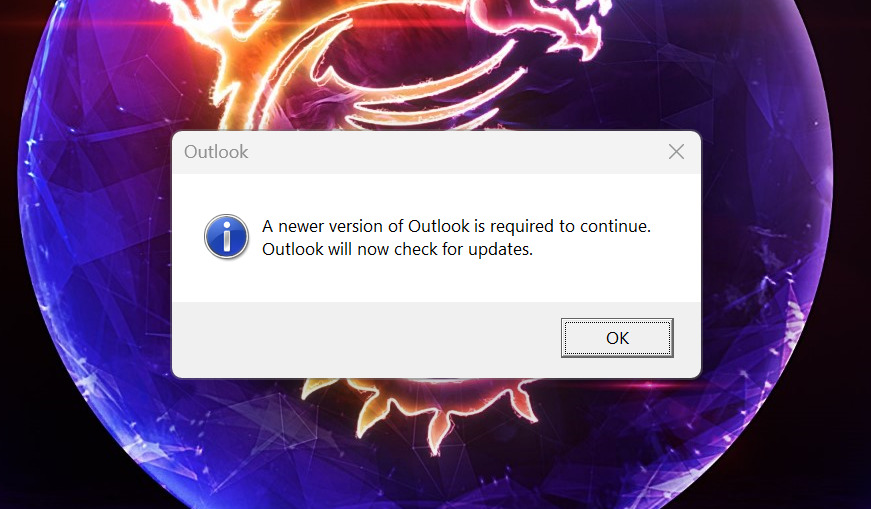
\includegraphics[width=0.5\linewidth]{visuals/outlook_requires_update.jpeg}
    \caption{Error Message after executing Forwarding Payload on MSI laptop}
    \label{fig:builtInTeensy}
    \cite{farhiMalboardNovelUser2019}
\end{figure}


Another big challenge with this payload is its UI focus. It requires a lot of settings menu navigation which is very time sensitive. Short delays are detrimental here. Even for the MSI laptop which has the most compute of the tested devices, an especially long delay for opening Outlook and a delay of around 300ms between every navigation step is necessary to ensure that every TAB and ARROW input is correctly placed. \\
On the microsoft surface laptop, the attack worked as expected, which can be attributed to the fact that it was built while continuously being tested on this device. For none of the other test objects did the payload work out of the box, each would require updates, new logins or even lack the new Outlook completely. 

The conclusion for this payload is that it is not versatile and indeed requires a rather specific set of circumstances to work. Its UI focus make this even harder, since delays have to be high to accommodate long the long loading times of an application like Outlook. If it works correctly, however, the payload can be very powerful and useful for gathering intelligence. 


\subsubsection{Disable Windows Event Logging}

GOAL: Disable Windows Event logging to hide possible traces another attack might leave. \\
PREREQUISITES: Windows 11

This payload has two versions; UI and CLI based approaches, as discussed in chapter \ref{Implementation}. For the UI based version, the usual problems occur; loading times, pop up problems, unforseen reactions by the host. However, since this time the payload navigates through Windows Settings panels and not Outlook, some more continuity and speed can be expected. There are no server calls to be made that influence loading times, instead the process should be more straight forward. 
The Command Line Version should be even more reliable. It contains fewer steps and therefore less margin for error. It is expected to run smoothly on all test subjects.

The first execution of the UI based approach proved once again its flakiness; Disabling Widows event logging on the MSI laptop would have evidently also stopped another process, which caused the pop up to confirm. This was not foreseen by the payload and therefore interrupted the process to the point where it exited the settings panel by selecting 'cancel' instead of 'apply' thereby ruining it's progress. A second execution successfully stopped windows event logging, since the pop up did not appear again. However, it failed to close the settings winows, leaving a trail of the attack. The navigation on the other side, was more reliable than what could be observed with the email forwarding payload which is as expected. \\
What was unexpected were language setting problems. When testing the payload on the TODO gaming desktop, it ran into problems because the search did not yield windows event logging, but instead 'Windows Defendeer Advanced'. The payload would had to be adjusted to find the german 'Windows-Ereignisprotokoll'. After this adjustment however, the next problem occurred; since the User did not have administrator rights, the settings options were greyed out and the payload had no chance of succeeding. \\
The payload worked well on the Surface Latoptop, as expected, since it was developed on it.

The CLI approach yielded much better results succeeding on the first try on the MSI laptop. As well as working on the custom built gaming computer after adjusting the payload to enter the administrator password. As expected it also worked well on the Microsoft Surface Laptop. This result solidifies the superiority of a command line approach as opposed to navigating user interfaces. 


Conclusively it can be said that this payload works very well when applying the CLI approach. The UI version can work as well, but requires a lot of fine tuning, administrator access, and English as system language. 



\subsubsection{Extract SSH hashes}

GOAL:\\ Extract SSH hashes from a default storage on a device and send them to a command and control (C\&C) server.
PREREQUISITES: Windows 11 and a running C\&C server, in this case Dropbox. Administrator rights are required

Since this script is working with defaults Windows settings, there are not a lot of challenges to be expected. On the MSI laptop it worked flawlessly, after some adjusting on the delays for opening the terminal. Since administrator access is not a given on the custom gaming computer, the payload had to be adjusted to include the administrator password. With this adjustment it was able to run successfully. The best results were again on the Windows Surface Latop, where it executed flawlessly. 


\subsubsection{{Extract Private Key Files}

GOAL: Find files that have extensions commonly used for private key files and send them to a C\&C server. \\
PREREQUISITES: Knowledge about the file system

This payload needs an entry point, some path to a local folder from which it can search through the files. If this is chosen too generally there may be permission issues. The entry point also heavily influences the time this payload takes to execute since it determines how many files the loop has to go through. The longer the script takes to execute, the easier it is to spot. \\
Since this payload does not require admin privileges one challenging step of opening an admin terminal is eliminated. One unexpected factor for errors is the validity length for the Dropbox access token. It expires within 4 hours. This means that in between saving the payload to the cable and the execution not more than those few hours may elapse. It was not a problem to adjust the payload for manual testing, however, this eliminates a C\&C server like Dropbox for boot scripts with unknown execution times. \\

The payload generally worked well on the Microsoft Surface laptop; it's file system is known and an adequate entry point could be chosen. The execution was a success on the MSI laptop and the custom desktop as well. These good results could be due to the fact that apart from starting PowerShell, there are no loading times that can throw off the execution of the payload. Even waiting for the loop to end was not a problem; although delays were not adjusted to the expected search time, PowerShell still recognized and executed the command after finishing the loop.



\subsubsection{Steal Web Session Cookies}

GOAL: Figure out the default browser of the target, then steal the websession cookies. \\
PREREQUISITES: None

This payload is pretty straight forward and simple. Nevertheless, challenges for it's flexibility arise. Executing the payload on the Microsoft Surface device went expectedly well, however, upon execution on the MSI laptop an error message occurred. Although the default browser on both of these devices is set to Firefox, their versions differ. While the Surface latptop had a slightly older version ( 129.0.1) the MSI laptop ran on the newest release, 129.0.2. This reflects in the path to their cookies file. The .2 version stores the cookies at '\\Mozilla\\Firefox\\Profiles\\dpsymep9.default-release\\cookies.sqlite'  while .1 stores them at 'Mozilla\\Firefox\\Profiles\\umva4gfp.default-release\\cookies.sqlite' . This unexpected little, but crucial detail, derailed the exectuion of the script on the MSI laptop. The chrome cookies path seems to be more robust; it worked without adjustments after changing the default for the MSI laptop to Chrome. 


GOAL:\\
PREREQUISITES:


\subsection{Specific Usecases}

gaming

\subsection{Windows 10 Home}




\section{Defence}
